
\section{Felder und Zeiger}

Wir haben bisher zwar schon die \verb|scanf| Funktion benutzt, aber noch nicht erklärt, wie sie funktioniert. 
Oder, genauer gesagt, wir haben noch nichts dazu gesagt, was \verb|&n| eigentlich bedeutet. 
Der Rest von \verb|scanf| sollte eigentlich von der Benutzung von \verb|printf| klar sein.

Um das verstehen zu können, muss man sich zunächst noch einmal ins Gedächtnis rufen, das eine Variable im Prinzip aus zwei Dingen besteht:
Einserseits dem Typ der Variablen und andererseits der Speicheradresse, unter der ein Wert abgelegt wird.
Über den Typ der Variablen weiss ich, wie viele bits im Speicher belegt sind, und wenn man die Anfangsadresse für das erste bit kennt, dann kann die gesamte Anzahl an bits auslesen und entsprechend dem Typ interpretieren.
C erlaubt Zugriff sowohl auf den Wert einer Variablen, als auch auf die Adresse, an der der Wert abgelegt ist.
Unterschieden wird zwischen den beiden mit dem \verb|&| operator. 
Für eine variable \verb|n| representiert \verb|n| den Wert und \verb|&n| die Speicheradresse.
Bei \verb|&n| spricht man auch von Zeiger (\emph{pointer}) und bei \verb|&| vom Adressenoperator.

Die Funktion \verb|scanf| verlangt nun als zweites Argument einen Zeiger.
Der Typ wird in der Zeichenkette angegeben, so dass die Funktion unter der Adresse, die mit \verb|&| angegeben wird, den Wert ablegen kann.

Da Zeiger in C eine sehr wichtige Rolle spielt, gibt es für sie spezielle Datentypen:
\begin{lstlisting}
  int n = 3;      // eine Variable vom Typ int
  int* address;  // eine Variable vom Typ Zeiger auf int
  address = &n;   // address zeigt auf n
  *address = 5;   // *address representiert den Wert, der unter der
                  // Adresse address gespeichert ist.
                  // man spricht von dereferenzieren
  n == 5;         // ist jetzt wahr.
\end{lstlisting}
Genauso gibt es einen Typ Zeiger auf \verb|double|, nämlich \verb|double*| und so weiter.
\begin{myblock}{Definition \texttt{Zeiger}}
Ein Zeiger ist eine Variable, die eine Adresse zusammen mit einem Datentyp speichert.
\end{myblock}
Um die Nützlichkeit von Zeigern zu veranschaulichen, führen wir zunächst Funktionen ein.
Eine Funktion kenne wir schon, das ist \verb|main|.
Eine beliebige Funktion wird nun über einen Namen, einen Rückgabewert und Eingangsparameter definiert.
Im folgenden Bespiel definieren wir eine Funktion, die zwei Parameter \verb|a, b| übergeben bekommt und diese um eins erhöht. 
Anschließend sollen diese beiden neuen Werte zurückgegeben werden.
Die Funktion hat aber nur einen Rückgabewert.

Ein Weg, um dieses Problem zu lösen, ist das sogenannte \emph{call by reference}.
Was \textbf{nicht} funktioniert ist das folgende:
\begin{lstlisting}
#include<stdio.h>
  // einfache Funktion um a,b um 1 zu erhoehen
  int increment( int a, int b) { 
    a++;
    b++;
    return(0);
  }
  
  int main(){
    int a = 2, b = 3;
    int ret = 0;
    printf("Wert vor der Funktion a=%d, b=%d\n", a,b);
    ret = increment(a, b); // die Variablen in unserem Block werden 
                            // nicht veraendert!
    printf("Wert nach der Funktion a=%d, b=%d\n", a, b); 
    return(ret);
  }
\end{lstlisting}
Der Grund ist, dass in der Funktion \verb|increment| neue Variablen \verb|a, b| angelegt werden, die nur in der Funktion selbst sichtbar sind. 
Sie haben also nichts mit den Variablen \verb|a, b| in der Funktion \verb|main| gemein, außer dem Namen.
Man spricht hier von \emph{call by value}, da die Variablen \verb|a, b| in der Funktion \verb|increment| mit den Werten der Variablen aus \verb|main| initialisiert werden.
Deswegen liefern die \verb|printf| Aufrufe in den Zeilen $12$ und $15$ das gleiche Ergebnis.
Denn die Variablen \verb|a, b| in \verb|main| wurden nicht verändert.

Bei \emph{call by reference} wird an Stelle des Wertes die Adresse übergeben.
\begin{lstlisting}
#include<stdio.h>
  // einfache Funktion um a,b um 1 zu erhoehen
  int increment(int* a, int* b) { 
    (*a)++;
    (*b)++;
    return(0);
  }
  
  int main(){
    int a = 2, b = 3;
    int ret = 0;
    printf("Wert vor der Funktion a=%d, b=%d\n", a,b);
    ret = increment(&a, &b); // die Variablen in unserem Block werden 
                            // nicht veraendert!
    printf("Wert nach der Funktion a=%d, b=%d\n", a, b); 
    return(ret);
  }
\end{lstlisting}
Die Funktion bekommt also zwei Parameter vom Typ \verb|int*|, also Zeiger auf \verb|int|. 
Dann wird mit dem Dereferenzierungsoperator \verb|*| der Wert, der unter den beiden Adressen gespeichert ist, um eins erhöht.
Das geschieht unter der Annahme, dass dort eine Variable vom Typ \verb|int| abegelegt ist.
Damit werden also direkt die Werte der Variable \verb|a, b| in \verb|main| verändert.

Zeiger kann man genau wie andere Variablen nutzen (womit auch klar ist, dass man auch Zeiger auf Zeiger definieren kann).
Folgendes Beispiel illustriert die Nutzung noch einmal, wobei \emph{NULL} der Nullzeiger ist:
\begin{lstlisting}
#include<stdio.h>

int main(){
   int  q = 10;
   int* p = NULL;
   p = &q;
   printf("Der Wert an der Adresse p ist:%d\n", *p);
   return(0);
}
\end{lstlisting}
In der vierten Zeile haben wir eine Variable vom Typ \verb|int| deklariert und mit dem Wert $10$ initialisiert, in der fünften Zeile eine Variable vom Typ \verb|int*|, die mit dem \verb|NULL| Zeiger initialisiert wurde.
in der sechsten Zeile wird dann \verb|p| auf die Adresse von \verb|q| gesetzt. 
Damit liefert die Dereferenzierung von \verb|p|, also \verb|*p|, den Wert von \verb|q|.
Dies ist in Abbildung \ref{pointfig} illustriert.
Zeigern dürfen nur gültige Adressen zugewiesen werden.
Dies kann allerdings, bis auf Ausnahmen, nicht vom Compiler überprüft werden.
Wenn doch keine gültige Adresse zugewiesen wurde, bekommt man den \emph{segmentation fault} als Laufzeitfehler.
Dieser Quelltext weisst sehr wahrscheinlich eine ungültige Adresse zu
\begin{lstlisting}
int *p=42;
\end{lstlisting}
allerdings wird im diesen Fall der Compiler sehr wahrscheinlich\footnote{Hängt leider vom Compiler ab} eine Warnung geben, denn $42$ ist vom Typ \verb|int|, und nicht vom Typ \verb|int*|. 
Wenn der Compiler sich hier nicht beschwert, sollte man die Dokumentation studieren, um heraus zu finden, wie man diesen Typ von Warnung anschalten kann, oder, wenn das nicht möglich ist, den Compiler wechseln.



\begin{figure}[!ht]
\centering
% Generated with LaTeXDraw 2.0.8
% Thu Feb 23 15:10:59 CET 2017
% \usepackage[usenames,dvipsnames]{pstricks}
% \usepackage{epsfig}
% \usepackage{pst-grad} % For gradients
% \usepackage{pst-plot} % For axes
\scalebox{0.5} % Change this value to rescale the drawing.
{
\begin{pspicture}(0,-8.856719)(29.2,8.8767185)
%\usefont{T1}{ptm}{m}{n}
%\rput(3.9903126,-0.7267187){0x7ffc5a48eb88}
%\usefont{T1}{ptm}{m}{n}
%\rput(16.572031,-0.7267187){0x7ffc5a4860aa}
%\usefont{T1}{ptm}{m}{n}
\psframe[linewidth=0.04,dimen=outer](29.2,-1.8367188)(0.0,-5.6367188)
%\psframe[linewidth=0.04,dimen=outer](2.6,-6.436719)(0.2,-8.636719)
%\psframe[linewidth=0.04,dimen=outer](4.8,-6.436719)(2.6,-8.636719)
\psline[linewidth=0.04cm](2.4,-1.8367188)(2.4,-5.6367188)
\psline[linewidth=0.04cm](4.9,-1.8367188)(4.9,-5.6367188)
\psline[linewidth=0.04cm](6.4,-1.8367188)(6.4,-5.6367188)
\psline[linewidth=0.04cm](7.8,-1.8367188)(7.8,-5.6367188)
\psline[linewidth=0.04cm](9.6,-1.8367188)(9.6,-5.6367188)
\psline[linewidth=0.04cm](11.2,-1.8367188)(11.2,-5.6367188)
\psline[linewidth=0.04cm](12.6,-1.8367188)(12.6,-5.6367188)
\psline[linewidth=0.04cm](14.0,-1.8367188)(14.0,-5.6367188)
\psline[linewidth=0.04cm](15.2,-1.8367188)(15.2,-5.6367188)
\psline[linewidth=0.04cm](17.0,-1.8367188)(17.0,-5.6367188)
\psline[linewidth=0.04cm](19.0,-1.8367188)(19.0,-5.6367188)
\psline[linewidth=0.04cm](21.0,-1.8367188)(21.0,-5.6367188)
\psline[linewidth=0.04cm](23.4,-1.8367188)(23.4,-5.6367188)
\psline[linewidth=0.04cm](26.0,-1.8367188)(26.0,-5.6367188)
%\usefont{T1}{ptm}{m}{n}
\rput(3.3576562,-2.7267187){int *}
%\usefont{T1}{ptm}{m}{n}
\rput(21.80922,-2.7267187){int}
%\usefont{T1}{ptm}{m}{n}
\rput(22.20922,-3.3267188){Name: q}
%\usefont{T1}{ptm}{m}{n}
\rput(22.011922,-4.1967187){Wert:}
\rput(21.80922,-4.67185){10}

%\usefont{T1}{ptm}{m}{n}
\rput(22.190312,-5.9267187){0x7ffc5a48eb88}
%\usefont{T1}{ptm}{m}{n}
\rput(3.7720314,-5.826719){0x7ffc5a4860aa}
%\usefont{T1}{ptm}{m}{n}
\rput(3.5867188,-3.3267188){Name: p}
%\usefont{T1}{ptm}{m}{n}
\rput(3.3267188,-4.19267187){Wert:}
%\usefont{T1}{ptm}{m}{n}
\rput(3.6267188,-4.67185){0x7ffc5a48eb88}
\pscustom[linewidth=0.04]
{
\newpath
\moveto(5.0,-6.2367187)
\lineto(5.3,-6.6367188)
\curveto(5.45,-6.8367186)(5.75,-7.1367188)(5.9,-7.2367187)
\curveto(6.05,-7.3367186)(6.4,-7.4867187)(6.6,-7.536719)
\curveto(6.8,-7.5867186)(7.2,-7.7367187)(7.4,-7.8367186)
\curveto(7.6,-7.936719)(8.0,-8.086719)(8.2,-8.136719)
\curveto(8.4,-8.186719)(8.8,-8.286718)(9.0,-8.336719)
\curveto(9.2,-8.386719)(9.65,-8.436719)(9.9,-8.436719)
\curveto(10.15,-8.436719)(10.6,-8.486719)(10.8,-8.536718)
\curveto(11.0,-8.586719)(11.45,-8.686719)(11.7,-8.736719)
\curveto(11.95,-8.786718)(12.45,-8.836719)(12.7,-8.836719)
\curveto(12.95,-8.836719)(13.45,-8.836719)(13.7,-8.836719)
\curveto(13.95,-8.836719)(14.4,-8.786718)(14.6,-8.736719)
\curveto(14.8,-8.686719)(15.25,-8.636719)(15.5,-8.636719)
\curveto(15.75,-8.636719)(16.25,-8.536718)(16.5,-8.436719)
\curveto(16.75,-8.336719)(17.25,-8.186719)(17.5,-8.136719)
\curveto(17.75,-8.086719)(18.15,-7.936719)(18.3,-7.8367186)
\curveto(18.45,-7.7367187)(18.8,-7.536719)(19.0,-7.436719)
\curveto(19.2,-7.3367186)(19.6,-7.1367188)(19.8,-7.036719)
\curveto(20.0,-6.936719)(20.4,-6.686719)(20.6,-6.536719)
}
\pscustom[linewidth=0.04]
{
\newpath
\moveto(19.0,-6.6367188)
\lineto(19.5,-6.6367188)
\curveto(19.75,-6.6367188)(20.15,-6.6367188)(20.3,-6.6367188)
\curveto(20.45,-6.6367188)(20.6,-6.5867186)(20.6,-6.436719)
}
\pscustom[linewidth=0.04]
{
\newpath
\moveto(19.8,-7.6367188)
\lineto(20.0,-7.1367188)
\curveto(20.1,-6.8867188)(20.3,-6.686719)(20.4,-6.7367187)
}
%\usefont{T1}{ptm}{m}{n}
\rput(14.13625,-7.9267187){*p liefert den Wert von q}
\pscustom[linewidth=0.04]
{
\newpath
\moveto(22.0,-1.2367188)
\lineto(21.8,-0.93671876)
\curveto(21.7,-0.7867187)(21.5,-0.48671874)(21.4,-0.33671874)
\curveto(21.3,-0.18671875)(21.05,0.11328125)(20.9,0.26328126)
\curveto(20.75,0.41328126)(20.5,0.7132813)(20.4,0.86328125)
\curveto(20.3,1.0132812)(20.05,1.2632812)(19.9,1.3632812)
\curveto(19.75,1.4632813)(19.4,1.6132812)(19.2,1.6632812)
\curveto(19.0,1.7132813)(18.6,1.8132813)(18.4,1.8632812)
\curveto(18.2,1.9132812)(17.75,1.9632813)(17.5,1.9632813)
\curveto(17.25,1.9632813)(16.8,2.0132813)(16.6,2.0632813)
\curveto(16.4,2.1132812)(15.95,2.2132812)(15.7,2.2632813)
\curveto(15.45,2.3132813)(15.0,2.4632812)(14.8,2.5632813)
\curveto(14.6,2.6632812)(14.15,2.7632813)(13.9,2.7632813)
\curveto(13.65,2.7632813)(13.15,2.8132813)(12.9,2.8632812)
\curveto(12.65,2.9132812)(12.15,3.0132813)(11.9,3.0632813)
\curveto(11.65,3.1132812)(11.15,3.1632812)(10.9,3.1632812)
\curveto(10.65,3.1632812)(10.2,3.0632813)(10.0,2.9632812)
\curveto(9.8,2.8632812)(9.4,2.7132812)(9.2,2.6632812)
\curveto(9.0,2.6132812)(8.55,2.5132813)(8.3,2.4632812)
\curveto(8.05,2.4132812)(7.6,2.2632813)(7.4,2.1632812)
\curveto(7.2,2.0632813)(6.8,1.7132813)(6.6,1.4632813)
\curveto(6.4,1.2132813)(6.0,0.86328125)(5.8,0.7632812)
\curveto(5.6,0.66328126)(5.25,0.46328124)(5.1,0.36328125)
\curveto(4.95,0.26328126)(4.7,0.01328125)(4.6,-0.13671875)
\curveto(4.5,-0.28671876)(4.2,-0.58671874)(4.0,-0.7367188)
\curveto(3.8,-0.88671875)(3.55,-1.1367188)(3.4,-1.4367187)
}
\pscustom[linewidth=0.04]
{
\newpath
\moveto(3.4,-1.4367187)
\lineto(3.5,-0.93671876)
\curveto(3.55,-0.68671876)(3.6,-0.28671876)(3.6,0.16328125)
}
\pscustom[linewidth=0.04]
{
\newpath
\moveto(3.4,-1.4367187)
\lineto(3.9,-1.3367188)
\curveto(4.15,-1.2867187)(4.55,-1.1867187)(5.0,-1.0367187)
}
%\usefont{T1}{ptm}{m}{n}
\rput(12.740937,3.8732812){\&q liefert den Wert von p}
\end{pspicture} 
}
\caption{\label{pointfig} Illustration Zeiger.}
\end{figure}

Zeiger sind in C doppelt wichtig, denn das wichtige Konstrukt von Feldern wird mit Hilfe von Zeigern realisiert. 
Für unser Sortierbeispiel möchten wir beispielsweise nicht $n$ Variablen mit verschiedenen Namen \verb|a1|, \verb|a2|, ... deklarieren.
Das wäre nicht nur ästetisch unschön, sondern auch extrem unpraktisch.
Wie sollte man diese Variablennamen zum Beispiel in einer Schleife in Abhängigkeit von der Schleifenvariablen ansprechen?
Deshalb stellt C Felder, sogenannte \emph{arrays} zur Verfügung.
Normalweise wenn wir Zahlen sortieren möchten, möchten wir nicht jeden Zahl, als
ein einzige Variable definieren. Auf diesem Fall gibt uns die Sprache die Arrays 
strukturen. Die Arrays bestehen aus mehreren nacheinander stehenden elementare 
Variablen mit den gleichen Datatypen. Für Indizierung mann muss
die Eckige Klammer verwenden. 
\begin{myblock}{Definition \texttt{Array}}
Ein Array ist eine Sammlung von Datenelementen vom gleichen Typ. Die 
Indizierung des Arrays geschieht mit positiven ganzen Zahlen von 0 bis Länge des Arrays minus eins.
\end{myblock}
Die Länge des Arrays muss zur Zeit der Übersetzung bekannt sein.
Im Beispiel sieht das wie folgt aus: 
\begin{lstlisting}
  #include<stdio.h>
  
  int main(){
    const int n = 4;
    int array1[] = {1,2,3,4}; // Deklaration und Initialisierung
    int array2[n];            // Deklaration, nicht initialisiert
    array2[0] = 1;            // Zuweisung einzelner Elemente
    array2[1] = 2;
    array2[2] = 3;
    array2[3] = 4;
    return(0);
  }
\end{lstlisting}
Hierbei wurden zwei \emph{int} Arrays erzeugt.
Beide haben die Länge $4$.
Die Länge des zweiten Arrays wurde mit Hilfe einer konstanten Variablen angegeben.
Alternativ kann man auch direkt $4$ schreiben.
Auf die einzelnen Elemente des Arrays wird mit Hilfe des \verb|[]| Operators zugegriffen.
Man beachte, dass die Indizes bei $0$ anfangen, und bis $3$, also Länge des Arrays minus 1, laufen. 

Die Benutzung von Arrays wird in folgendem Beispiel illustriert:
\begin{myexampleprogram}{Beispiel: \texttt{Näherung von $\pi$}}
  In diesem Beispiel berechnen wir $\pi$ näherungsweise.
  Dafür verwenden wir folgende Integraldarstellung von $\pi$:
  \begin{equation}
    \pi=4\cdot \int_{0}^{1} \mathrm{d}x \dfrac{1}{1+x^2}
  \end{equation}
  Das Integral berechnen wir numerisch, indem wir die Fläche unterhalb der Kurve als eine Summe abschätzen. 
  Dabei bedienen wir uns der sogenannten Trapez-Regel.
  Wir teilen das Interval $[0,1]$ in $N$ gleichlange Unterintervalle auf.
  Den jeweilige linke Punkt des Intervals nennen wir $x_i$, $i=0,...,N$, wobei $x_n-x_{n-1}=\Delta=\mathrm{const}$.
  Auf jedem Unterintervall approximieren wir die Funktion linear, wie in folgender Abbildung dargestellt ist:
  \vspace{-5cm}
  \begin{center}
    %\begin{minipage}
    \includegraphics[width=.8\linewidth]{trapez1.ps}
%    \caption{Funktion $\drac{1}{1+x^2}$ und der Trapez-Regel\label{trapezrul}}
  \end{center}
  \vspace{-6cm}
  In unserem Fall sind die Punkte wie folgt gegeben
  \begin{displaymath}
    x_i = i/N\,,\qquad i = 0, ..., N-1\,.
  \end{displaymath}
  \textbf{Put a proper bounding box!!}
  Definieren wir folgende Funktion
  \[
  f(x) = \frac{1}{1+x^2}\,,
  \]
  so können wir wie folgt über die Teilergebnisse summieren:
  \begin{equation}
    \int_{0}^{1} \mathrm{d}x \dfrac{1}{1+x^2}\approx \sum_{i=0}^{N-1}\frac{1}{2N}[f(x_i)+f(x_{i+1})]
  \end{equation}
  Hier ist der entsprechende C Quelltext, der Arrays benutzt:
  \begin{lstlisting}
    #include<stdio.h>
    const int MAX=10000;

    int main(){
      int N=0;
      double f[MAX], x[MAX]; // double arrays der Laenge MAX
      scanf("%d",&N);
      // Pruefe die Eingabe
      if (N >= MAX) {
        printf("Fehler, zu vielen Stuetzstellen\n");
        return(-1);
      }
      if (N < 0) {
        printf("N muss groesser als 0 sein!\n");
        return(-2);
      }
      for (int i = 0; i < N; ++i){
        x[i] = (double) i/(double) N;
        f[i] = 1./(1 + x[i]*x[i]);
      }
      double summe = 0.;
      for (int i = 0; i < N-1; ++i) {
        summe += (f[i] + f[i+1]);
      }
      summe += f[N-1] + 0.5; // Randterm
      printf("Die Naeherung von pi ist =%e\n", 2./N*summe);
      return(0);
    }
  \end{lstlisting}
  Neben der Benutzung von Arrays, haben wir noch ein weiteres neues Konzept eingeführt.
  Bei der Division von $i/N$, beide vom Typ \verb|int|, in Zeile $10$ haben wir einen expliziten \emph{cast} nach \verb|double| durchgeführt, damit keine Division ganzer Zahlen durchgeführt wird.
  
  Dieses Beispiel hätten wir natürlich auch ohne Arrays durchführen können, aber es illustriert deren Benutzung.
\end{myexampleprogram}
Zum Indexoperator \verb|[]| ist es sehr wichtig zu wissen, dass dabei nicht überprüft wird, ob der Index größer ist, als die Länge des Arrays.
Folgendes geht also im Prinzip
\begin{lstlisting}
  int list[5];
  int i = 5;
  list[i] = 3;
\end{lstlisting}
und wird vom Compiler übersetzt. 
Im besten Fall erhält man dann bei der Ausführung dieses Codes einen \emph{segmentation fault}.
Im schlechtesten Fall ist \verb|list[5]| Speicher, auf den das Programm zugreifen kann.
Dann erhält man keinen Laufzeitfehler und modifiziert ungewollt Speicher, den man nicht modifizieren will.
Dies kann zu sehr seltsamem Verhalten des Programms führen, und das Finden eines solchen Fehlers ist sehr schwierig.
Deshalb sollte man Indizierungen immer mit großer Sorgfalt überprüfen.

\subsection{Zeichenketten oder Strings}

In C gibt es keinen elementaren Datentyp für Zeichenketten, sogenannte \emph{strings}.
Zeichenkette werden mit Hilfe von Arrays abgebildet.
Ein Zeichen kann in einer Variablen vom Typ \verb|char| gespeichert werden, siehe ASCII Zeichensatz.
Eine Zeichenkette kann also durch eine Array von Elementen vom Typ \verb|char| erzeugt werden.
Das Ende einer Zeichenkette wird durch das Zeichen \verb|\0| angegeben.
Im nächsten Beispiel lesen wir eine Zeichenkette von der standard Eingabe ein, bis wir das Zeichen fuer das Ende des Strings finden und testen, ob die Kette eine Zahl enthält:
\begin{lstlisting}
#include<stdio.h>
const int MAX_LENGTH = 1000;
const int TRUE = 1;
const int FALSE = 0;

int main(){
   char string[MAX_LENGTH];
   int i=0;
   char a;
   int ergebnis = FALSE;
   scanf("%s", string);
   while(1) {
     if (string[i] == '\0')
       break;
     if ( (string[i] >= '0') && ( string[i] <= '9') )
       ergebnis = TRUE;
     i++;
   }
   if(ergebnis) printf("Der String %s enthaelt Zahlen\n", string);
   else printf("Der String enthaelt keine Zahlen\n");
   return(0);
}
\end{lstlisting}
Es wird zunächst eine Zeichenkette über die Tastatur eingelesen.
Offensichtlich ist \verb|string| ohne den Indexoperator \verb|[]| vom Typ \verb|char*|, also Zeiger auf \verb|char|. 
Dann nutzen wir eine \verb|while| Schleife mit konstant wahrem logischem Ausdruck.
Die Schleife wird dann mit \verb|break| abgebrochen, wenn das Endstring Zeichen gefunden wurde.
In der Schleife wird dann jedes Element der Kette darauf überprüft, ob es eine Zahl ist.
Dementsprechend wird die Variable \verb|ergebnis| gesetzt.

Vielleicht ist es Ihnen schon aufgefallen, aber der obige Beispielquelltext ist nicht sauber programmiert.
Der Grund ist die Tatsache, dass wir die Länge des eingelesenen Strings nicht überprüfen, und damit nicht wissen, ob die maximale Länge überschritten wurde, oder nicht.
Es kommt zu einem sogenannten \emph{buffer overflow}.
Im besten Fall bekommt man bei einem zu langen Array einen Laufzeitfehler. 
Im schlechtesten Fall kann man allerdings in Speicher schreiben, der dafür nicht vorgesehen ist.
Es sollte also auf jeden Fall eine solche Überprüfung vorgenommen werden!

\subsection{Zeigerarithmetik}

Man kann auch eine Zeichenkette initialisieren:
\begin{lstlisting}
  #include<stdio.h>
  int main(){
    char string[]={'H','e','l','l','o',' ','w','o','r','l','d','\0'};
    char *pointer = NULL;
    pointer = &string[6];
    printf("Das siebte Zeichen im String ist %c\n",*pointer);
    return(0);
  }
\end{lstlisting} 
und dann mit \verb|pointer| auf einzelne Elemente der Zeichekette zugreifen.
Das ist nicht nur ein alternativer Weg, um auf die Elemente eines Arrays zuzugreifen.
C stellt Zeiger intern als ganze Zahlen dar und auf jedem Zeigetyp sind auch arithmetische Operationen definiert.
Beispielsweise ist folgendes in C korrekter Quelltext:
\begin{lstlisting}
  int list[5];
  int * plist = NULL;
  plist = list; // equivalent zu plist = &list[0];
  for(int i = 0; i < 5; i++) {
    *plist = i;
    plistx++;  // equivalent zu plist = plist + 1; oder plist += 1;
  }
\end{lstlisting}
Mit unserer bisherigen Kenntnis des Operators \verb|++|, würden wir erwarten, dass der Wert von \verb|plist| um eins erhöht wird.
Das ist im Prinzip auch richtig, allerdings findet die Erhöhung in Einheiten der Länge des Typs, auf den der Zeiger zeigt.
Und damit zeigt \verb|plist++| auf das nächste Element in der Liste \verb|list|.
Denn C reserviert für \verb|int list[5];| einen zusammenhängenden Speicherbereich der Länge fünf mal Länge von \verb|int|.
\verb|list|, ohne den Indexoperator, ist selbst vom Typ \verb|int*|, und zeigt auf den Anfang dieses Speicherbereichs. 
\verb|list[3]| ist dann equivalent zu folgender Dereferenzierung: \verb|*(list + 3)|.
Und damit weisst obiger Beispielcode dem $i$ten Element von \verb|list| den Wert $i$ zu.
Im folgenden Beispiel finden sich einige der möglichen arithmetischen Operationen für Zeiger:
\begin{lstlisting}
  #include<stdio.h>

  int main(){
    int sqnum[] = {1,4,9,16,25,36,49};
    int *pointer;
    int *pointer2;
    pointer = sqnum;
    pointer++;
    printf("Nach der Inkrementierung des Zeigers %d\n", *pointer);
    pointer--;
    printf("Nach der Dekrementierung des Zeigers %d\n", *pointer);
    pointer += 2;
    printf("Nach dem Hinzufuegen von 2 zum Zeiger %d\n", *pointer);
    pointer -= 2;
    printf("Nach dem Subtrahieren von 2 vom Zeiger %d\n", *pointer);   
    ++pointer;
    pointer2 = &sqnum[4];
    printf("Zwischen pointer2 und pointer gibt es %ld Elemente\n",pointer2-pointer);
    return(0);
  }
\end{lstlisting}
Überlegen Sie Sich, was obiges Programm als Ausgabe erzeugen wird, bevor Sie diesen Quelltext übersetzen und ausführen lassen.
Die \verb|++| Operation auf einen Zeiger vom Typ \verb|int| ist in Abbildung~\ref{pointinc} illustriert.

\begin{figure}[!ht]
  \centering
  % Generated with LaTeXDraw 2.0.8
  % Sun Feb 26 08:55:41 CET 2017
  % \usepackage[usenames,dvipsnames]{pstricks}
  % \usepackage{epsfig}
  % \usepackage{pst-grad} % For gradients
  % \usepackage{pst-plot} % For axes
  \scalebox{0.5} % Change this value to rescale the drawing.
           {
             \begin{pspicture}(0,-2.6)(33.6,2.62)
               
               \pscustom[linewidth=0.04]
                        {
                          \newpath
                          \moveto(4.5,0.5)
                          %\lineto(7.5,1.5)
                          \curveto(4.5,1.5)(9.0,3.)(13.5,0.5)
                        }
                        \rput(8.5,2.4){\LARGE *Pointer}
                        
                        
                        \psframe[linewidth=0.04,dimen=outer]( 3,-0.8)( 0.,-2.6)
                        \rput(4.5,-2.9){0x7ffc3fa500aa}
                        \rput(4.5,-1.49){0x7ffc3fa5bd20}
                        \rput(4.5,0.0){\LARGE Pointer}
                        
                        \psframe[linewidth=0.04,dimen=outer]( 6,-0.8)( 3.,-2.6)
                        \psframe[linewidth=0.04,dimen=outer]( 9,-0.8)( 6.,-2.6)
                        \psframe[linewidth=0.04,dimen=outer](12,-0.8)( 9.,-2.6)
                        \rput(13.5,-1.49){\LARGE 1}
                        \psframe[linewidth=0.04,dimen=outer](15,-0.8)(12.,-2.6)
                        \rput(13.5,-2.9){0x7ffc3fa5bd20}
                        \rput(13.5,0.0){\LARGE sqnum[0]}
                        
                        
                        \rput(16.5,-1.49){\LARGE 4}
                        \psframe[linewidth=0.04,dimen=outer](18,-0.8)(15.,-2.6)
                        \rput(16.5,-2.9){0x7ffc3fa5bd24}
                        \rput(16.5,0.0){\LARGE sqnum[1]}
                        
                        
                        \rput(19.5,-1.49){\LARGE 9}
                        \psframe[linewidth=0.04,dimen=outer](21,-0.8)(18.,-2.6)
                        \rput(19.5,-2.9){0x7ffc3fa5bd28}
                        \rput(19.5,0.0){\LARGE sqnum[2]}
                        
                        
                        \rput(22.5,-1.49){\LARGE 16}
                        \psframe[linewidth=0.04,dimen=outer](24,-0.8)(21.,-2.6)
                        \rput(22.5,-2.9){0x7ffc3fa5bd32}
                        \rput(22.5,0.0){\LARGE sqnum[3]}
             \end{pspicture}
           }
           
           \vspace{1cm}
           \scalebox{0.5}{
             \begin{pspicture}(0,-2.6)(33.6,2.62)
               
               \pscustom[linewidth=0.04]
                        {
                          \newpath
                          \moveto(4.5,0.5)
                          %\lineto(7.5,1.5)
                          \curveto(4.5,1.5)(11.5,3.)(16.5,0.5)
                        }
                        \rput(8.5,2.4){\LARGE *Pointer}
                        
                        
                        \psframe[linewidth=0.04,dimen=outer]( 3,-0.8)( 0.,-2.6)
                        \rput(4.5,-2.9){0x7ffc3fa500aa}
                        \rput(4.5,-1.49){0x7ffc3fa5bd24}
                        \rput(4.5,0.0){\LARGE Pointer}
                        
                        \psframe[linewidth=0.04,dimen=outer]( 6,-0.8)( 3.,-2.6)
                        \psframe[linewidth=0.04,dimen=outer]( 9,-0.8)( 6.,-2.6)
                        \psframe[linewidth=0.04,dimen=outer](12,-0.8)( 9.,-2.6)
                        \rput(13.5,-1.49){\LARGE 1}
                        \psframe[linewidth=0.04,dimen=outer](15,-0.8)(12.,-2.6)
                        \rput(13.5,-2.9){0x7ffc3fa5bd20}
                        \rput(13.5,0.0){\LARGE sqnum[0]}
                        
                        
                        \rput(16.5,-1.49){\LARGE 4}
                        \psframe[linewidth=0.04,dimen=outer](18,-0.8)(15.,-2.6)
                        \rput(16.5,-2.9){0x7ffc3fa5bd24}
                        \rput(16.5,0.0){\LARGE sqnum[1]}
                        
                        
                        \rput(19.5,-1.49){\LARGE 9}
                        \psframe[linewidth=0.04,dimen=outer](21,-0.8)(18.,-2.6)
                        \rput(19.5,-2.9){0x7ffc3fa5bd28}
                        \rput(19.5,0.0){\LARGE sqnum[2]}
                        
                        
                        \rput(22.5,-1.49){\LARGE 16}
                        \psframe[linewidth=0.04,dimen=outer](24,-0.8)(21.,-2.6)
                        \rput(22.5,-2.9){0x7ffc3fa5bd32}
                        \rput(22.5,0.0){\LARGE sqnum[3]}
                        
             \end{pspicture} 
           }
           \caption{\label{pointinc} Illustration zur Inkrementieren eines Zeigers von Typ int. Oben vor der Inkrementierung, unten nach der Inkrementierung.}
\end{figure}

An dieser Stelle müssen wir auf einen möglichen Fehler hinweisen.
Folgender Quelltext wird vom Compiler anstandslos übersetzt
\begin{lstlisting}
  int main() {
    int list[5];                      // int array
    double * plist = (double *) list; // explizit cast
    *(plist + 1) = 3;
    return(0);
  }
\end{lstlisting}
Wenn man Zeile $3$ durch
\begin{lstlisting}
  double * plist = list; // without cast
\end{lstlisting}
übersetzen das die meisten Compiler auch noch, hoffentlich wenigstens mit einer Warnung.
Was ist problematisch an obigen Code:
\verb|plist + 1| zeigt nicht auf das zweite Element in \verb|list|.
Denn die Länge von \verb|double| und \verb|int| ist nicht identisch.
Da \verb|plist| vom Typ Zeiger auf \verb|double| ist, bedeutet \verb|plist + 1| dass die entsprechende Adresse um die Länge von \verb|double| erhöht wird.
Damit ist aber der Speicherbereicht von \verb|list| nicht mehr als \verb|int| interpretierbar.
Obiger Code wird also undefiniertes Verhalten nach sich ziehen!

Zusammenfassend können wir also die Elemente eines Arrays auf zwei verschiedene Art und Weisen indizieren
\begin{enumerate}
\item mit dem Indexoperator \verb|[]|.
\item mit arithmetischen Operationen.
\end{enumerate}
Wie schon gesagt, intern behandelt C ein Array quasi als einen Zeiger.
Es gibt aber wichtige Unterschiede.
Wenn \verb|array| als Array deklariert ist, so darf man dessen Adresse nicht veraendern.
Folgendes Bespiel erläutert dies:
\begin{lstlisting}
#include<stdio.h>
int main(){
   int *pointer;
   int array[]={1,4,9,16,25,36,49,64};
   int i=2;
   pointer = array; // pointer zeigt auf &array[0]
   printf("Die Werte sind identisch: %d %d\n",array[i], *(pointer+i));
   pointer++;       // sinnvoll
   array++;         // nicht erlaubt!
   array=pointer;   // nicht erlaubt!
}
\end{lstlisting}

\textbf{ist das folgende sinnvoll hier zu machen!?} 
Es gibt eine weitere Unstershied in Bezug auf char Arrays und Pointers auf char. Lassen
Sie uns das folgende Beispiel sehen:
\begin{lstlisting}
  #include<stdio.h>
  int main(){
    char array[]="Hello world";
    char *pointer="Hello world";
    array[1] = 'a';   // korrekt
    pointer[1] = 'a'; // uebersetzt, fuehrt aber zu einem segmentation fault!
    return(0);
  }
\end{lstlisting}
In der dritten Zeile wir definieren ein Zeichenarray, damit wir also fur 12 Zeichen Speicherzellen reservieren. 
In den vierten Zeile wir definieren nur ein Pointer, und die Zeichenkette "Hello world" wird in einer konstanter
Speicherplatz speichern. Der Pointer will nur zeigt auf deiser konstanter Speicherplatz. Das bedeutet durch den
Pointer wir natürlich wir können nicht ändern der Wert der Variable von einem konstanten Spiecherplatz. Im gegenteil
wenn wir Array verwenden, wir können ihrer Elementen natürlich ändern.

Können wir auch vergleichoperatoren auf Pointers verwenden. Nur auf den Pointer macht es ziemlich kein Sinn.
Selbst wenn die Werte von zwei Variablen gleich ist, wahrseinlich haben Sie unterschiedlich Adresse in Speicherplatz.
Allerdings mit der Dereferenzierung Operator kann mann alle Vergleichungsoperator verwenden. Wenn die Pointer nicht
auf demselben Objekten zeigen, ob größer oder kleiner der Wert des Pointers gibt es uns keine Information. 
Üblicherweise vergleichen wir Pointers nur mit dem NULL pointer. Zum Beispiel wir den können NULL pointer 
verwenden um eine Fehler die Anwälden zu berichten.

Um die Bedeutung des Types vom Pointer noch einmal zu betonen, wir schließen noch ein Beispiel ein.
Hier wir wollen die erste und zweite halb-Teil ein Variable von Typ $int$ haben. Wir erreichen es
durch Pointers auf $short~int$ type. Anweisungen zwischen unterschiedlichen Pointer Typen sind nicht möglich.
Zum Beispiel wir können nicht direkt ein Wert von Pointer int Typ zu ein Pointer von shot int Type weisen.
Das können wir durch Typ casting. Wir zeigen diese Fall in der siebten Zeile. Wenn wir dann in der
neunten Zeile der Pointer inkremenentieren, er will nicht auf den nächsten int typ zeigen, sonder auch
auf der nächsten $short~int$ Typ, was tatsächlich in unserem Bespiel das zweite Halfe einer int Variable
ist. Nocheinmal, wenn wir einen Verschiebung zu einem Pointer hinfügen, der Pointer will zeigt auf die Variable
deren Adresse mit dem Größe von Pointer mal die Verschiebung von der Basisadresse ist.

\begin{lstlisting}
#include<stdio.h>
int main(){
   int *pointer, zahl=0x0002000F;
   short int *pointers;
   printf("Zahl is %d %x \n",zahl,zahl);
   pointer=&zahl;
   pointers=(short int *)pointer;
   printf("Der Wert der ersten Half  %x\n",*pointers);
   printf("Der Wert der zweiten Half ist %x\n", *(pointers+1));
}
\end{lstlisting}


\endinput
